\documentclass[a4paper,12pt]{article} % This defines the style of your paper

\usepackage[top = 2.5cm, bottom = 2.5cm, left = 2.5cm, right = 2.5cm]{geometry} 

\usepackage[T2A]{fontenc}
\usepackage[utf8]{inputenc}
\usepackage[russian]{babel}

\usepackage{multirow} 
\usepackage{booktabs} 

\usepackage{graphicx} 

\usepackage{setspace}
\setlength{\parindent}{0in}

\usepackage{float}

\usepackage{amsmath}

\usepackage{fancyhdr}

\usepackage{pgfplots}
\pgfplotsset{compat=1.9}

\pagestyle{fancy} 

\fancyhf{} 

\lhead{\footnotesize Расчетное задание №13}

\rhead{\footnotesize Николаев Юрий} 

\cfoot{\footnotesize \thepage} 

\begin{document}

\thispagestyle{empty} 

\begin{tabular}{p{15.5cm}} 
НИУ МЭИ \\ А-13а-19  \\ Вариант 13 \\ Николаев Юрий\\
\hline 
\\
\end{tabular} 

\vspace*{0.3cm}

\begin{center} 
	{\Large \bf Расчетное задание №13} 
	\vspace{2mm}
\end{center}  

\vspace{0.4cm}


\section{Задание}
Функция $y = y(x)$ задана таблицей своих значений. Применяя метод наименьших квадратов, приблизить функцию многочленами 1-й и 2-й степеней. Для каждого приближения определить величину среднеквадратичной погрешности. Построить на одном чертеже точечный график функции и графики многочленов.

\begin{center}
\begin{tabular}{| c | c | c | c | c | c |}
\hline
    x & -5,2 & -2,6 & 0 & 2,6 & 5,2 \\ \hline
    y & -1,7 & -3,4 & -4,7 & -4,8 & -8 \\
\hline
\end{tabular}
\end{center}

\section{Решение}

\begin{enumerate}

\item Найдем $P_0(x) = a_0$:

$a_0 = \frac{-1,7 - 3,4 - 4,7 - 4,8 - 8}{5} = -4,52$

\item Приблизим функцию многочленом 1-ой степени $P_1(x) = a_0 + a_1x$, $m = 1$:

Нормальная система наименьших приближений квадратов при этом имеет вид:
$$
\begin{cases}
    s_0 a_0 + s_1 a_1 = b_0 \\
    s_1 a_0 + s_2 a_1 = b_1 \\
\end{cases}
$$
Вычислим коэффициенты системы: 
\begin{center}
    $s_0 = \sum_{i = 0}^{n} x_i^0 = 5 $;

    $s_1 = \sum_{i = 0}^{n} x_i^1 = 0 $;

    $s_2 = \sum_{i = 0}^{n} x_i^2 = 67,6 $;

    $b_0 = \sum_{i = 0}^{4} y_i \cdot x_i^0 = -22,6 $;

    $b_1 = \sum_{i = 0}^{4} y_i \cdot x_i^1 = -36,4 $
\end{center}

Тогда система имеет вид:
$
\begin{cases}
    5a_0 + 0a_1 = -22,6 \\
    0a_0 + 67,6a_1 = -36,4  \\
\end{cases}
$

Решаем систему и получим многочлен: $P_1(x) = -4,52 - 0,54x$

\begin{center}
    $P_1(-5,2) = -1,712$; 
    
    $P_1(-2,6) = -3,116$; 
    
    $P_1(0) = -4,52$;
    
    $P_1(2,6) = -5,924$; 
    
    $P_1(5,2) = -7,328$
\end{center}

Найдем среднеквадратичное отклонение:
$$
    \begin{gathered}
        \sigma(P_1, f) = \sqrt{\frac{1}{5} \sum_{i = 0}^4(P(x_i) - f_i)^2} = \\ \sqrt{\frac{1}{5} [(-0,012)^2 + (-0,284)^2 + (0,18)^2 + (-1,124)^2 + (0,672)^2]} = 0,6047
    \end{gathered}
$$

\item Приблизим функцию многочленом 2-ой степени $P_2(x) = a_0 + a_1x + a_2x^2$, $m = 2$:

Нормальная система наименьших квадратов при этом примет вид:

$$
\begin{cases}
    s_0 a_0 + s_1 a_1 + s_2 a_2 = b_0 \\
    s_1 a_0 + s_2 a_1 + s_3 a_2 = b_1 \\
    s_2 a_0 + s_3 a_1 + s_4 a_2 = b_2 \\
\end{cases}
$$

Вычислим недостающие коэффициенты системы: 
\begin{center}
    $s_3 = \sum_{i = 0}^{n}x_i^3 = 0$
    
    $s_4 = \sum_{i = 0}^{n}x_i^4 = 1553,72$
    
    $b_2 = \sum_{i = 0}^{4} y_i \cdot x_i^2 = -317,72$
\end{center}

Тогда система имеент вид:
$
\begin{cases}
    5a_0 + 0a_1 + 67,6a_2 = -22,6 \\
    0 a_0 + 67,6a_1 + 0a_2 = -36,4 \\
    67,6a_0 + 0a_1 + 1553,72a_2 = -317,72 \\
\end{cases}
$

Решаем систему и получим многочлен: $P_2(x) = -4,262818 - 0,538462x - 0,019022x^2$
\begin{center}
    $P_2(-5,2) = -1,9772$; 

    $P_2(-2,6) = -2,9914$; 

    $P_2(0) = -4,262818$

    $P_2(2,6) = -5,7914$; 

    $P_2(5,2) = -7,5772$
\end{center}

Тогда среднеквадратичное отклонение: $\sigma(P_2, f) = 0,5651$

\begin{figure}[h]
\center{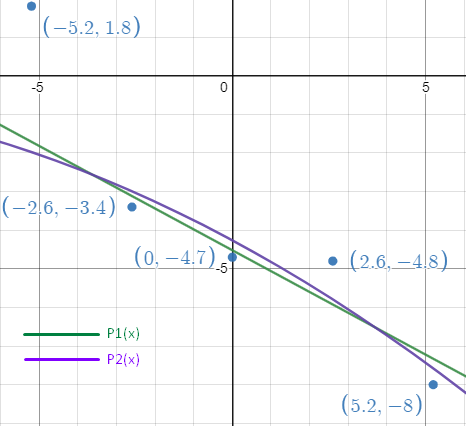
\includegraphics[scale=1.2]{graphic.png}}
\caption{График}
\label{fig:image}
\end{figure}


\end{enumerate}

\end{document}